\section{Plataforma de desarrollo y validación}
\label{sec:ana_mininet_wifi}

En este punto se va a valorar que plataforma se va a utilizar para desarrollar y validar el protocolo de comunicación in-band. Lo primera cuestión que se tiene que tener en cuenta cuando se va a elegir una plataforma de este tipo es, ¿Vamos a simular o a emular?. Aunque mucha gente considera que estos términos son equivalentes, no son lo mismo. Cuando hablamos de simulación nos referimos a un software que calcula el resultado de un evento dado un comportamiento esperado, donde la escala de tiempos de la simulación no se corresponde con la realidad. Es decir, el proceso a simular puede tener una duración de dos horas, pero como lo que se gestionan son los eventos asociados al proceso, el tiempo de la simulación solo vendrá regido por lo que tarde en procesar dichos eventos. Por otro lado, la emulación recrea el escenario bajo estudio en su totalidad en un hardware específico para luego estudiar su comportamiento. Donde la escala de tiempos de la emulación es el mismo que el tiempo real del proceso a emular. Un ejemplo para diferenciar ambos podría ser pensar en la cabina de un avión. Si jugáramos a un videojuego como Flight Simulator\footnote{\url{https://www.flightsimulator.com/}} estaríamos simulando el vuelo, pero si practicáramos utilizando una escala 1:1 (Ver figura \ref{fig:emu_simu}) con controles reales estaríamos hablando entonces de emulación.\\

%fig 1
\begin{figure}[ht!]
    \centering
    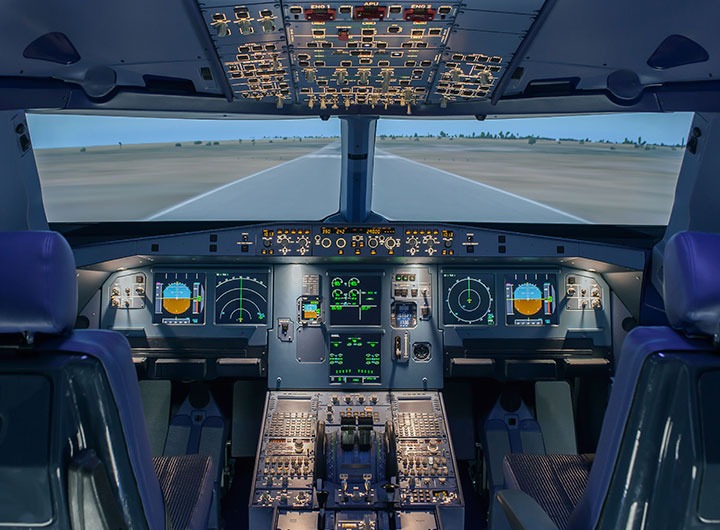
\includegraphics[width=0.8\textwidth]{archivos/img/analisis/emu_simu.jpeg}
    \caption{Entorno de emulación real de una cabina de avión a escala 1:1 \cite{emusim}}
    \label{fig:emu_simu}
\end{figure}

Una vez que ya tenemos claro cuales son las diferencias sobre la emulación y la simulación, vamos a ver que opciones tenemos en ambos ambitos para elegir una plataforma que se adecue a las necesidades del proyecto. De entre todas las opciones barajadas nos hemos quedados con las dos opciones en las cuales el autor tiene más experiencia, y en las cuales se pueden virtualizar enlaces inalambricos.

\begin{itemize}
    \item Contiki-ng haciendo uso de su simulador integrado llamado Cooja, explicado anteriormente en la sección \ref{sec:contikiNG} del estado del arte.

    \item Mininet-WiFi, explicado anteriormente en la sección \ref{subsec:mininetWIFIS} del estado del arte.
\end{itemize}